\begin{center}

  \begin{tabular}{rp{16cm}lp{20cm}}%{rl}

  % after \\: \hline or \cline{col1-col2} \cline{col3-col4} ...

  论文地址:& \href{https://arxiv.org/pdf/1606.07792v1.pdf}{https://arxiv.org/pdf/1606.07792v1.pdf} \\
  来源:& DLRS, 2016 \\
  作者:& Heng-Tze Cheng, Levent Koc, et al. \\

  源码:& \href{https://github.com/shenweichen/DeepCTR-Torch/blob/master/deepctr_torch/models/wdl.py}{Wide\&Deep} \\

%  slides:& \href{http://yunshengb.com/wp-content/uploads/2017/03/nips_2018_r2l_workshop_talk.pdf}{{\footnotesize Convolutional Set Matching for Graph Similarity}}\\

  关键词:& \textbf{Recommender systems} \\

  写于:& \date{2021-08-15}

  \end{tabular}

\end{center}

该论文\cite{cheng2016wide}提出了一个新的模型用于App推荐的模型 --- Wide\&Deep,该模型结合了Wide模型(LR模型)和Deep模型(Deep Neural Network)。

\paragraph{问题定义}
在推荐系统中有一个挑战 --- \textbf{Memorization \& Generalization}。Memorization:学习频繁共现的物品/特征在历史数据中的关系。Generalization:根据关系的传递性,探索新的特征组合,即使未在训练数据中出现或很少出现的特征组合也能给出合适的推荐。Memorization可以通过Wide模型来解决,Generalization可以通过Deep模型来解决。


\paragraph{Wide\&Deep}
\begin{figure}[h]
	\centering
	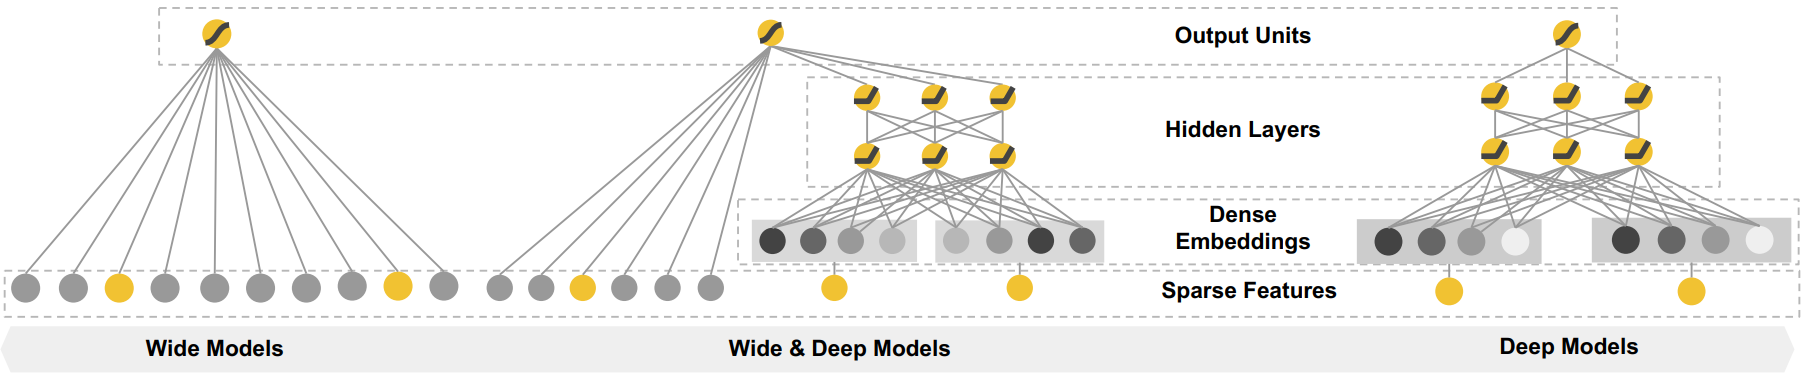
\includegraphics[width=.95\textwidth]{pics/wide&deep.png}
	\caption{Wide\&Deep}
	\label{fig:wdl}
\end{figure}

\subparagraph{Wide Component}
Wide模型一般是一个广义的线性模型,如LR或者包含特征交叉的线性模型。

\subparagraph{Deep Component}
Deep模型是一个基于神经网络的模型。在输入层,Deep模型将类别变量进行嵌入得到dense embedding(即Fig.\ref{fig:wdl}中的 Dense Embedding)。

\subparagraph{Joint of Wide and Deep}
Wide模型和Deep模型是联合训练的,Wide\&Deep模型的输出等于Wide和Deep模型的输出加权求和。论文中使用FTRL(Follow-the-regularized-leader,其在处理诸如逻辑回归之类的带非光滑正则化项,如L1范数的优化问题上性能非常出色)\cite{mcmahan2011follow-the-regularized-leader}来优化Wide\&Deep模型。

在论文中,作者将类被特征转化为ID,将连续值特征按照值的分位数转换到[0,1]。


\paragraph{总结}

\begin{itemize}
	\item Memorization与Generalization的结合
	\item Wide\&Deep用于Ranking
\end{itemize}

